\documentclass[12pt,a4paper]{article}
\usepackage[spanish]{babel} %Seteo el idioma
\usepackage[utf8]{inputenc} %Es para escribir con acentos
\usepackage{titling}
\usepackage{graphicx}



\begin{document}
%Defino el título y autores
\title{%
	Tópicos de Programación para Científicos Computacionales\\
	\large Informe del Trabajo Práctico Final}
	
\author {Eduador Agustín Rosselot$^{1-3}$ y Maximiliano Jose Perez Frasette$^{2-3}$\\ 
	\small{$^{1}$earosselot@gmail.com [924/11]}\\
	\small{$^{2}$maxi.perezfrasette@gmail.com [862/12]}\\
	\small{$^{3}$Grupo 1 - Alumnos de doctorado del Departamento de Geología}\\
	}
\date{Diciembre 2019}

\maketitle


\section{Ejercicio 1: Dividir y Conquistar}

El archivo donde se encuentran las implementaciones del ejercicio 1 está incluído en el repositorio con el nombre \textit{Ejercicio1.py}, dentro de la carpeta srcej\_1. En esa misma carpeta, se encuentra el gráfico generado (bajo el nombre de \textit{GraficoEj1.png})y un archivo llamado \textit{datosGrafico1.txt} , con los tiempos de cómputo obtenidos. También está incluído el archivo \textit{datitos.txt}, que son los datos suministrados junto con el tp.\par

El código donde están las funciones implementadas se encuentra divido en cuatro secciones. En la primer sección se encuentran las funciones principales, en la segunda sección están todas las funciones auxiliares necesarias para implementar las funciones principales. En la tercer sección se encuentran las funciones implementadas para analizar los diferentes tiempos de ejecución. Por último, en la cuarta sección están los comandos para obtener el gráfico. Cada sección está dividida por un comentario que las identifica claramente. \par

En la sección número uno están las tres funciones principales pedidas por el enunciado del tp, \texttt{listadepuntos(fn)}, \texttt{distanciaMinima(l)} y \texttt{distanciaMinimaDyC(l,algoritmo)}. La implementación de las primeras dos funciones es relativamente sencilla. \texttt{Listadepuntos(fn)} utiliza la función auxiliar \texttt{entero(a)}, que convierte \textit{strings} en \textit{floats}. \texttt{DistanciaMinima(l)} recibe una lista de tuplas e itera la cantidad de veces necesarias para calcular la distancia euclídea entre todos los puntos de la lista.Al finalizar, devuelve el par de puntos más cercanos. Está función necesita como parámetro una lista de al menos dos elementos, en ese caso devuelve ese par de puntos.Además, utiliza la función auxiliar \texttt{distancia(p1,p2)}, la cual calcula la distancia euclídea entre dos pares de coordenadas. Por último, \texttt{distanciaMinimaDyC(l, algoritmo)} también busca el par de puntos más cercano dentro de una lista de puntos l, pero utiliza la técnica de Dividir y Conquistar. Esta función está dividida en dos bloques. En el primer bloque, ordena a la lista de entrada "l" según la coordenada en x. Puede utilizar diferentes técnicas de ordenamiento, las cuales se pasan como argumento. Puede utilizar las técnicas de \textit{up-sort},\textit{merge-sort} o el algoritmo por default de python. Para las dos primeras técnicas de ordenamiento, se implementaron cuatro funciones auxiliares (las funciones maxPos(a,b,c) y upSort(l)para ordenar la lista según la técnica de \textit{up-sort} y  merge(l1,l2) y mergeSort(l) para ordenar la lista según la técnica de \textit{merge-sort}). En el segundo bloque, se hace el llamado de la función auxiliar \texttt{minimaDistRec(l)}, que calcula el par de puntos más cercanos de manera recursiva y según la técnica de divivir y conquistar. El parámetro de entrada l, debe ser una lista ordenada según la coordenadas en x. El ordenamiento se lleva a cabo dentro de \texttt{minimaDistanciaDyC(l,algoritmo)} para evitar ordenar una lista que ya está ordenada durante los pasos recursivos. Además, \texttt{minimaDistRec(l)} utiliza la función auxiliar \texttt{paresCruzados(l1,l2,x,dist)}. Está función auxiliar recibe dos pares de listas ordenadas en la coordenada x, que corresponden con los conjuntos de puntos de izquierda y derecha partidos en el paso de dividir.El punto x, mediante el cual se hizo la división y la minima distancia entre los pares de puntos de ambas listas. Está función implemente el paso de combinar, y devuelve posibles pares de coordenadas que podrían encontrarse a una distancia menor a la hallada hasta ese momento (mezcla pares de puntos de los grupos izquierda y derecha)\par 
En la tercera sección del código, se encuentran implementadas las funciones \texttt{puntosAleatorios(a,b)} y \texttt{experimentarAlgoritmos()}. La primer función genera un set de puntos de cantidad \"a\". Los posibles valores de las coordenadas varían  entre \"-b\" y \"b\". La segunda función testea a los algoritmo para diferentes sets de datos y devuelve un archivo .txt con los tiempos de ejecución de cada algoritmo. \par 

A continuación se presentan los gráficos de tiempos obtenidos para diferentes cantidades de datos y para diferentes algoritmos empleados. Se tomó como criterio analizar a partir de 1000 puntos, porque para cantidades menores la medición del tiempo está dentro del rango de error del módulo time de python. Las mediciones se emplearon varíando los sets de datos en orden creciente (se probó para 1000, 5000, 10000, 15000, 20000 y 50000 puntos, ver Figura 1). \par 
Como se observa en la Figura 1, a medida que crece el número de datos a calcular, la función más lenta es distanciaMinima(l), la cual utiliza fuerza bruta como algoritmo. Además, como estaba previsto, puede verse que aumenta exponencialmente (fuerza bruta es un algoritmo de O($n^{2}$)). Por otro lado, puede observarse que para la resolución del problema mediante la técnica de Dividir y Conquistar, los tiempos de computo disminuyen considerablemente (esta técnica tieme complejidad de O(n.log(n)). En particular, si el ordenamiento se lleva a cabo de acuerdo a la técnica de \textit{merge-sort} o mediante el algoritmo por \textit{default} de python, el algoritmo es más rápido que al utilizar el ordenamiento por \textit{up-sort}.

\section{Ejercicio 2: Python y Numba}





\section{Ejercicio 3: Backtraking}




\begin{figure}
  \centering
    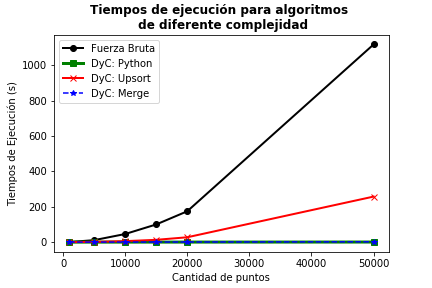
\includegraphics[width=0.8\textwidth]{GraficosEj1}
  \caption{Tiempos de ejecución obtenidos para los diferentes       algoritmos}
  \label{fig:ejemplo}
\end{figure}


\begin{figure}
  \centering
    \includegraphics[width=0.8\textwidth]{GráficosGray}
  \caption{Gráficos de escalabilidad para el filtro gray}
  \label{fig:ejemplo}
\end{figure}


\begin{figure}
  \centering
    \includegraphics[width=0.8\textwidth]{GráficosBlur}
  \caption{Gráficos de escalabilidad para el filtro blur}
  \label{fig:ejemplo}
\end{figure}

\end{document}
